\documentclass[tikz,convert={density=150,size=600,outext=.png}]{standalone}
\usetikzlibrary{shapes, calc, arrows, fit, positioning, decorations, patterns, decorations.pathreplacing, chains, snakes}

\begin{document}
  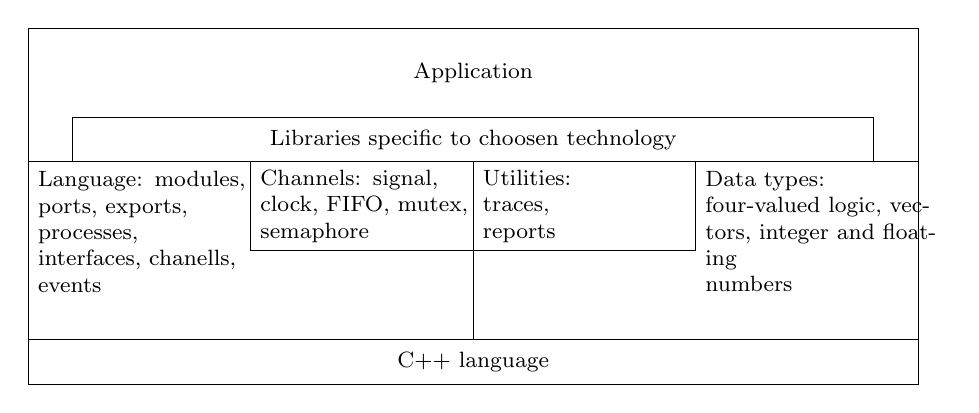
\begin{tikzpicture}[scale=1.13, >=latex, font=\footnotesize]
    \coordinate (a01) at (-5 ,0.5);
    \coordinate (a02) at ( 5 ,0.5);
    \coordinate (a03) at (-5  ,-1);
    \coordinate (a04) at (-2.5,-1);
    \coordinate (a05) at (   0,-1);
    \coordinate (a06) at ( 2.5,-1);
    \coordinate (a07) at (   5,-1);
    \coordinate (a08) at (   0,-2);
    \coordinate (a09) at (  -5,-3);
    \coordinate (a10) at (   0,-3);
    \coordinate (a11) at (   5,-3);
    \coordinate (a12) at (   5,-3.5);

    \coordinate (b01) at (-4.5,-0.5);
    \coordinate (b02) at ( 4.5,  -1);

    \coordinate (l01) at ( 0,   0);
    \coordinate (l02) at ( 0,-0.75);
    \coordinate (l03) at (-2.5,-1.5);
    \coordinate (l04) at ( 0,-1.5);
    \coordinate (l05) at (-5, -1);
    \coordinate (l06) at ( 2.5, -1);
    \coordinate (l07) at (   0,-3.25);

    \draw (a01) rectangle (a12);
    \draw (b01) rectangle (b02);

    \draw (a03) rectangle (a10);
    \draw (a04) rectangle (a08);

    \draw (a05) rectangle (a11);
    \draw (a08) rectangle (a06);
    \draw (a09) rectangle (a12);

    \node at (l01) {Application};
    \node at (l02) {Libraries specific to choosen technology};
    \node[align=left, text width=3cm, anchor = west] at (l03) {Channels: signal, clock, FIFO, mutex, semaphore};
    \node[align=left, text width=3cm, anchor = west] at (l04) {Utilities: \\ traces, \\ reports};

    \node[align=left, text width=3cm, anchor = north west] at (l05) {Language: modules, ports, exports,\\ processes,\\ interfaces, chanells, events};
    \node[align=left, text width=3cm, anchor = north west] at (l06) {Data types: \\ four-valued logic, vectors, integer and floating\\ numbers};

    \node at (l07) {C++ language};
  \end{tikzpicture}
\end{document}
